\section{Gateway Architecture}


\subsection{Request Flow}

\begin{figure}[h]
\centering
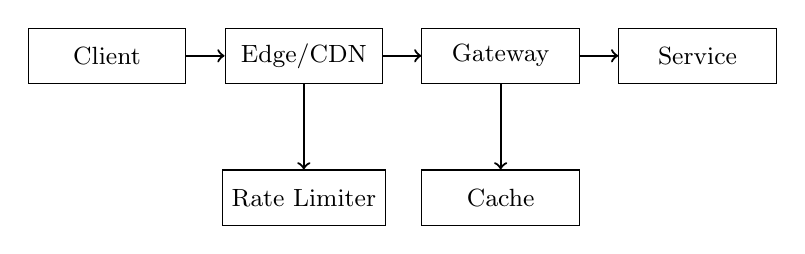
\begin{tikzpicture}[
    node distance=1.5cm,
    box/.style={rectangle, draw, minimum width=2cm, minimum height=0.7cm, font=\small},
    arrow/.style={->, thick}
]
    \node[box] (client) {Client};
    \node[box, right of=client, xshift=1cm] (edge) {Edge/CDN};
    \node[box, right of=edge, xshift=1cm] (gateway) {Gateway};
    \node[box, right of=gateway, xshift=1cm] (service) {Service};

    \node[box, below of=gateway, yshift=-0.3cm] (cache) {Cache};
    \node[box, below of=edge, yshift=-0.3cm] (ratelimit) {Rate Limiter};

    \draw[arrow] (client) -- (edge);
    \draw[arrow] (edge) -- (gateway);
    \draw[arrow] (gateway) -- (service);
    \draw[arrow] (gateway) -- (cache);
    \draw[arrow] (edge) -- (ratelimit);
\end{tikzpicture}
\caption{Gateway request flow}
\end{figure}

Request processing stages:

\begin{enumerate}
    \item \textbf{Edge}: TLS termination, DDoS protection, geographic routing
    \item \textbf{Authentication}: Validate credentials, extract identity
    \item \textbf{Rate Limiting}: Check and decrement quota
    \item \textbf{Cache Lookup}: Return cached response if valid
    \item \textbf{Routing}: Forward to appropriate backend service
    \item \textbf{Response Processing}: Transform, cache, return
\end{enumerate}

\subsection{Authentication}

\subsubsection{API Key Authentication}

\begin{lstlisting}[caption=API Key Header]
Authorization: Bearer sk_live_abc123...
\end{lstlisting}

API keys encode:
\begin{itemize}
    \item Key type: $\{sk\_live, sk\_test, pk\_live, pk\_test\}$
    \item Merchant identifier
    \item Permission scopes
    \item Expiration (optional)
\end{itemize}

\subsubsection{OAuth 2.0 for Third-Party Apps}

\begin{lstlisting}[caption=OAuth Token Request]
POST /oauth/token
Content-Type: application/x-www-form-urlencoded

grant_type=authorization_code
&code=AUTH_CODE
&client_id=CLIENT_ID
&client_secret=CLIENT_SECRET
&redirect_uri=https://app.example.com/callback
\end{lstlisting}

\subsubsection{Permission Model}

\begin{definition}[API Permission]
A permission $p$ is a tuple $(resource, action, scope)$ where:
\begin{itemize}
    \item $resource \in \mathcal{R}$: resource type
    \item $action \in \{read, write, delete\}$
    \item $scope \in \{own, all\}$: ownership constraint
\end{itemize}
\end{definition}

Permission check:
\begin{equation}
authorized(key, request) = \exists p \in permissions(key) : matches(p, request)
\end{equation}

